\documentclass[a4paper]{article}
\usepackage{tabularx}
\usepackage[english]{babel}
\usepackage[utf8]{inputenc}
\usepackage{amsmath,amsfonts}
\usepackage{mathrsfs}
\usepackage{graphicx}
\usepackage[colorinlistoftodos]{todonotes}
\usepackage[margin=1in]{geometry}
\usepackage{enumitem}
\usepackage[final]{hyperref}
\usepackage{bm}
\usepackage{caption,subcaption}
\usepackage{cite}
\hypersetup{
	colorlinks=true,       
	linkcolor=blue,        
	citecolor=blue,     
	filecolor=magenta,
	urlcolor=blue         
}
\bibliographystyle{unsrt}
\graphicspath{{../figures/}}

\title{Entropy change at the hard-disk melting transition}
\author{Buming Guo} 
\date{\today}

\begin{document}
\maketitle

Lossless data compression that approaches the minimum encoding limit of a data sequence can be used to describe the Shannon entropy, or the order of a system. The Computable Information Density (CID), which is given by the ratio of binary code length between the compressed and original sequence, has been successfully used to detect and quantize phase transitions of several non-equilibrium many-body systems\cite{2017arXiv170804993M}. 

Here we will examine a simple case of entropy-driven phase transition of hard-sphere from liquid to solid state, and see if the image compression scheme can find an abrupt change of CID that corresponds to the entropy behavior of the first-order phase transition.


\paragraph{Hard-disk melting transition}

Thermodynamics laws shows that the system will minimize its Helmholtz free energy $F = E - TS$ at constant volume and temperature, where $E$ is the internal energy consisting of kinetic part $K$ and potential part $U$. For hard-sphere case, the potential energy is either 0 or $\infty$, thus according to the configuration part of the partition function (proportional to free volume):
\begin{equation}
Q = \frac{1}{N!} \int_{0}^{L} \dotsm \int_{0}^{L} dx_1 \dotsm dx_{2N} ~\theta(x_1 \dotsm x_{2N})
\end{equation}
where the weight $\theta$ is 0 or 1 for configurations with and without overlap, the potential energy $U = - \frac{\partial \ln Q}{\partial \beta}$ gives zero, implying that the internal energy of hard-sphere system is just its kinetic energy, which is only a function of temperature. In this sense, at constant temperature, a phase transition is driven only by entropy. This therefore gives us a rather direct case to examine the data compression scheme.

\begin{figure}[ht]
	\centering
	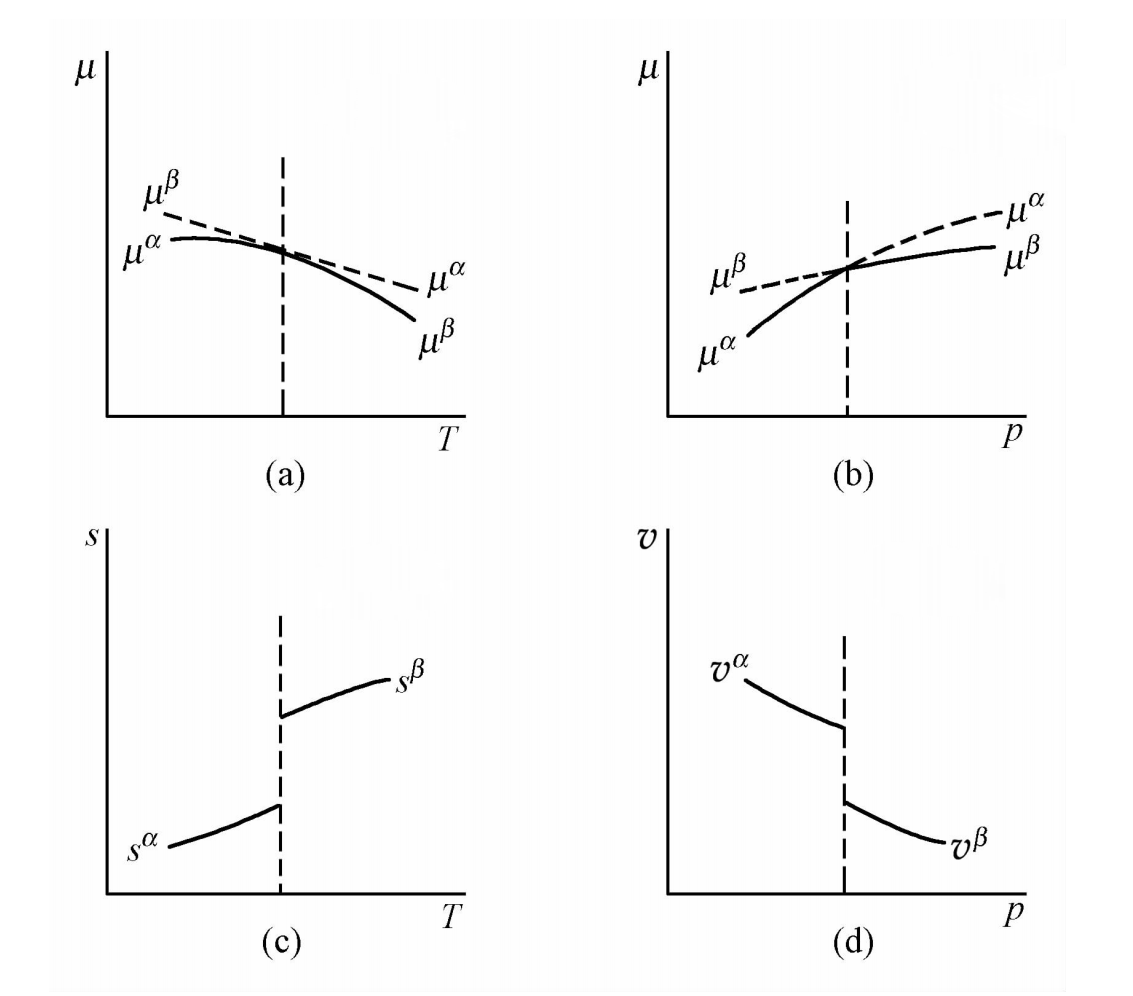
\includegraphics[width=0.64\linewidth]{transition.png}
	\caption{
		\cite{zonghanlin} Schematic plot of the first-order phase transition of Gibbs ensemble. The system will minimize its chemical potential and the first partial derivative of $\mu$, which correspond to entropy and volume, undergo discontinuous change.
	}
	\label{fig:transition}
\end{figure}

In thermodynamics, a first order phase transition is characterized by a discontinuity of the partial derivative of the chemical potential in Gibbs ensembles. As illustrated in Fig.\ref{fig:transition}, the system goes from one phase $\alpha$ to anther phase $\beta$ with minimal chemical potential, and the entropy and volume per mol:
\begin{equation}
s=-\left(\frac{\partial \mu}{\partial T}\right)_p, ~~ v=\left(\frac{\partial \mu}{\partial p}\right)_T
\end{equation}
undergo discontinuous change at the transition. For hard-disk case specifically, this correspond to the jump of volume when crossing the transition by varying pressure. With $G=E-TS+pV$ and the continuous change of G and p, the entropy S should be discontinuous due to the abrupt change of density. However, it is hard to do MC simulation with constant pressure especially in parallel, so we use NVT ensemble instead with large particle number N by convention, where the entropy is continuous as a function of $\phi$. As NVT and NPT ensembles are equivalent at thermodynamic limit, we can simply replace the control variable to pressure calculated from our constant-NV ensemble, and we should expect a jump of entropy.


\paragraph{Equation of state}

To determine the phase transition, we need to calculate the equation of state $p(\phi)$ for hard-disk fluid. We generate ensemble samplings of configuration at each volume fraction $\phi$ using HOOMD-blue that can run Monte Carlo on GPU in large scale. The pressure is carried out with\cite{PhysRevE.87.042134}
\begin{equation} \label{eq:pressure}
\beta p = \frac{\partial \ln Q}{\partial V} = \frac{N}{V} \left[ 1 + 2 \phi ~ g(2\sigma_+) \right] ,
\end{equation}
where $\sigma$ is the radius of the disk and $g(2\sigma_+)$ represents the pair-correlation function $g(r)$ at the point of contact. 

Fig.\ref{fig:p_phi} shows the equation of state of a hard-disk system with number of particles $N=256^2$ near the melting transition region. The pressure is calculated through the pair correlation function at the point of contact as in Eqn.\ref{eq:pressure}. Each point in the figure is the time average of $10^8$ time steps after relaxation of $2 \times 10^7$ steps, where a time step here correspond to approximately 4 Monte Carlo sweeps of the entire system in 2D due to the checkerboard decomposition scheme used in the GPU MC algorithm MPMC \cite{ANDERSON201327}. 

\begin{figure}[ht]
	\centering
	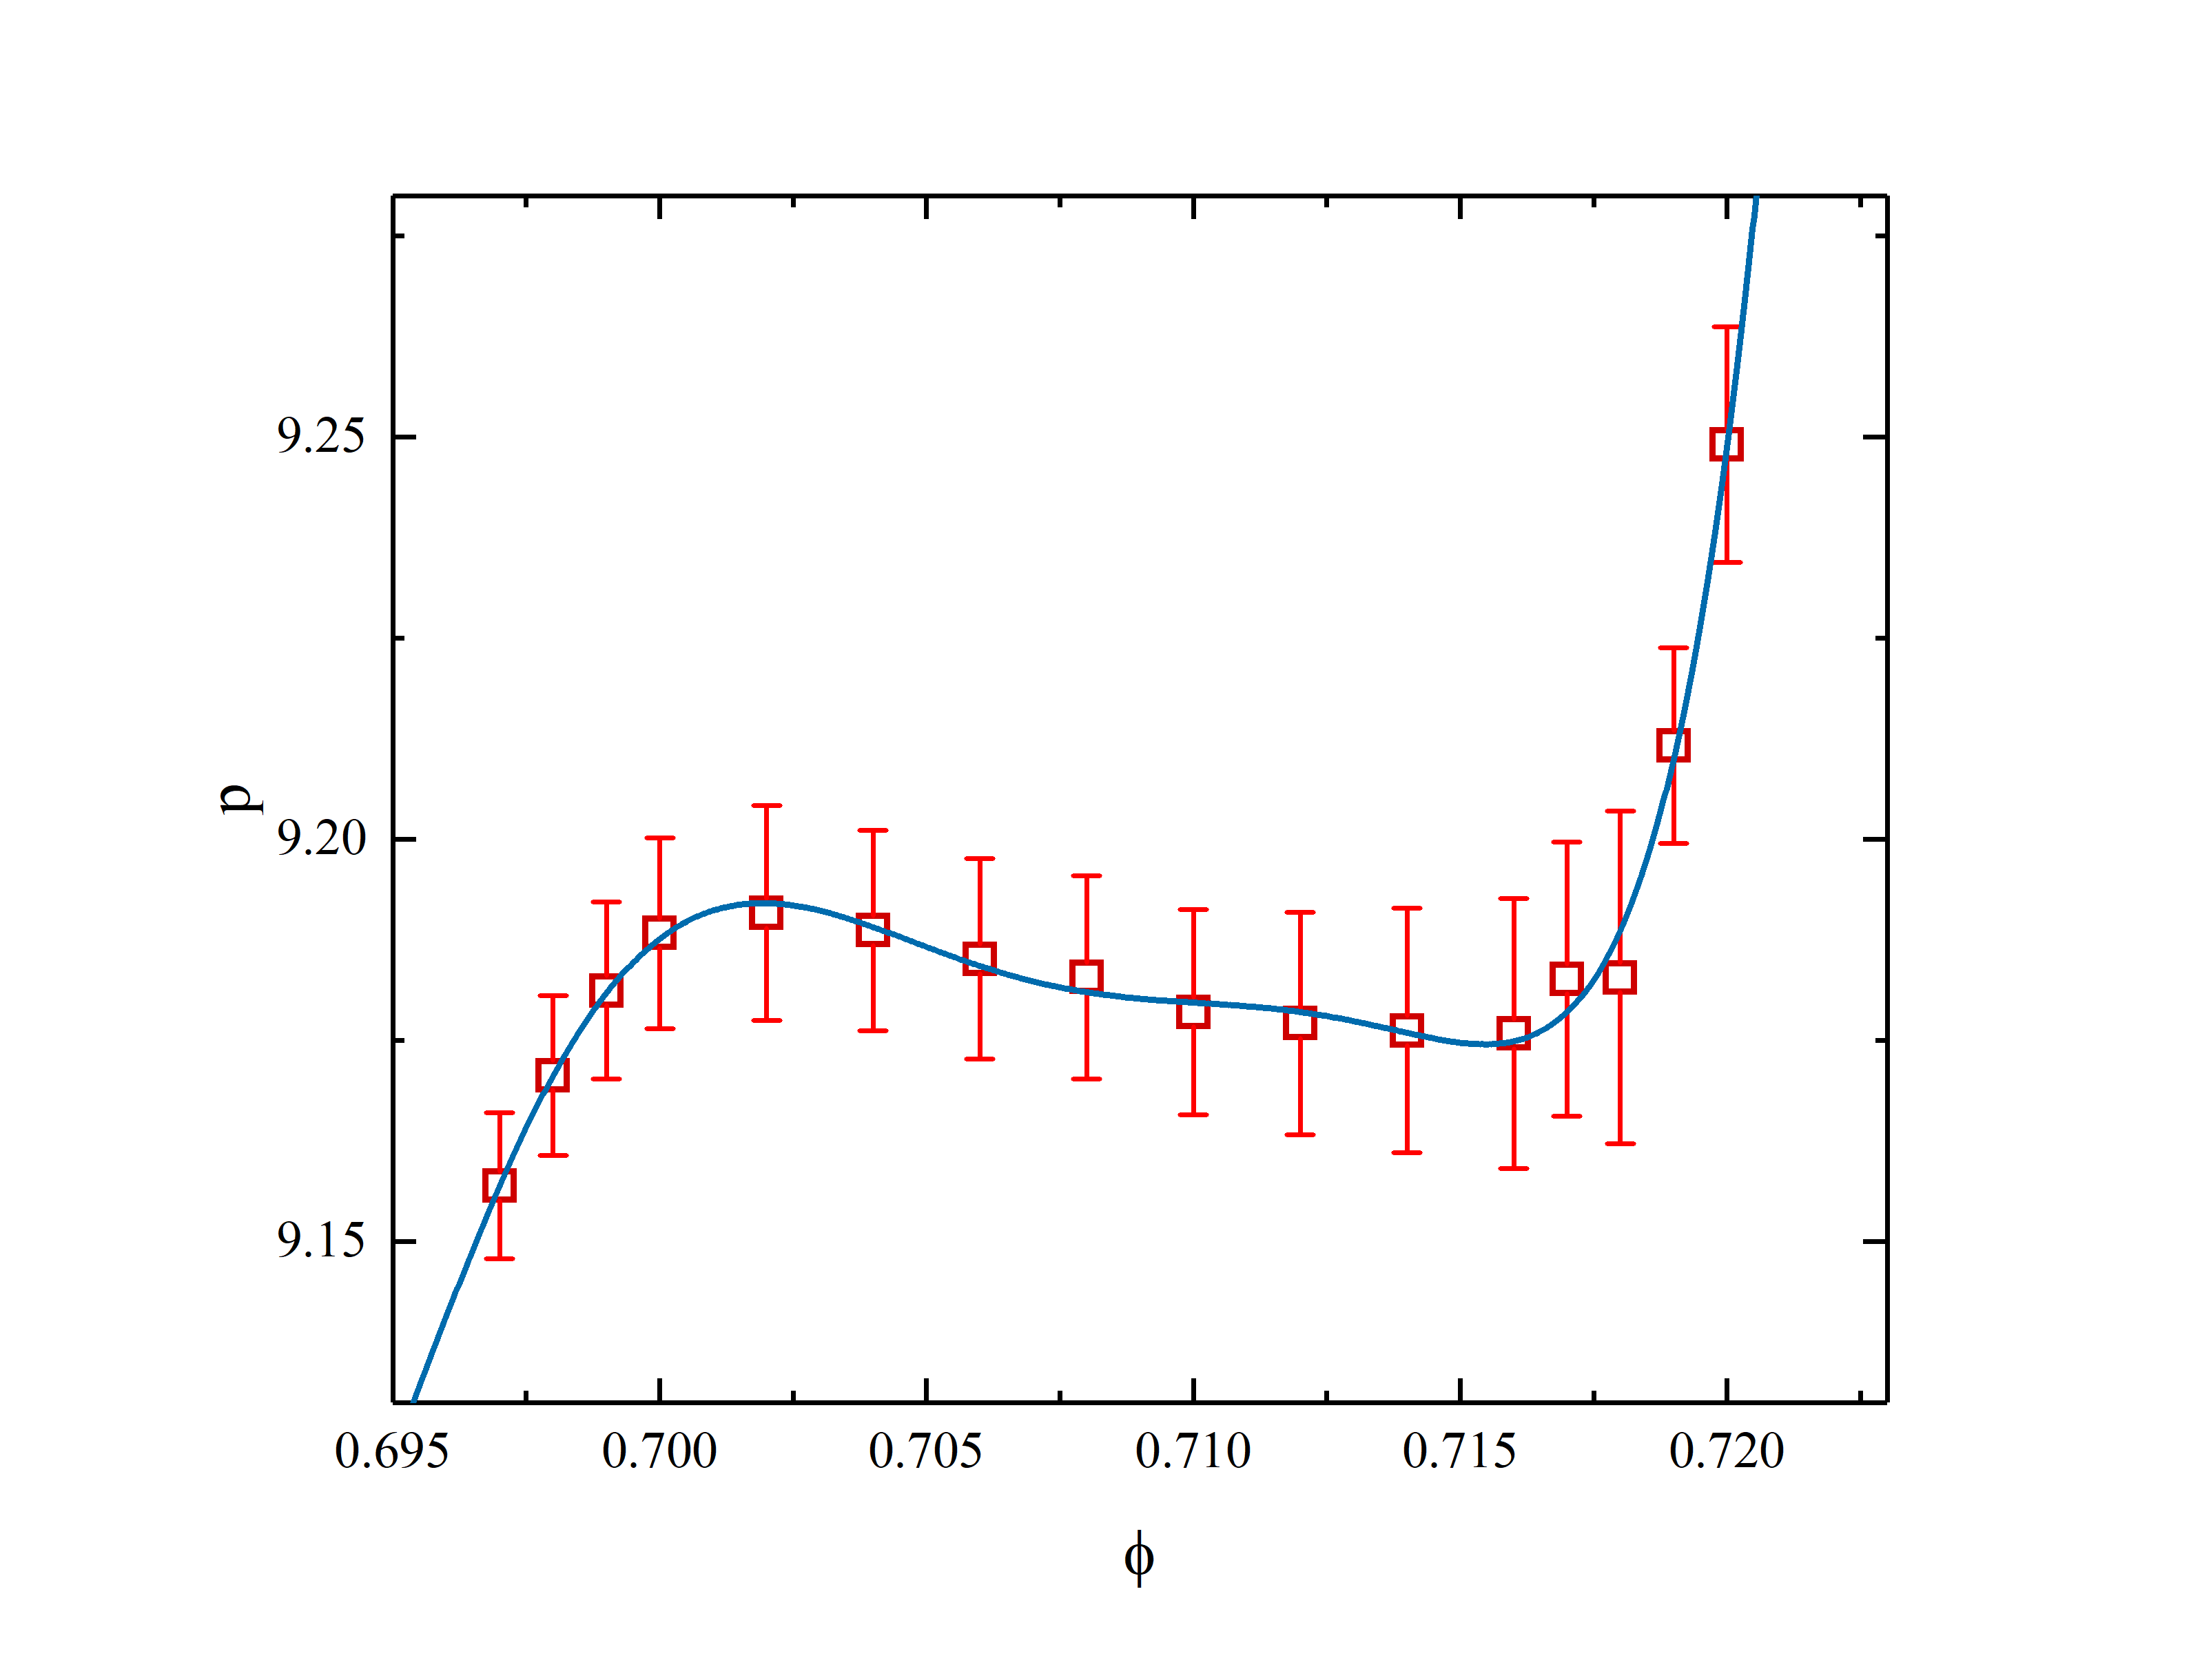
\includegraphics[width=0.7\linewidth]{p_phi.png}
	\caption{
		The equation of state of the $N=256^2$ hard-disk system. Points are time averaged pressure with error bar of standard deviation. The blue line is the 6th-order polynomial fit of the $p-\phi$ data points, where $\phi$ is the volume fraction.
	}
	\label{fig:p_phi}
\end{figure}

As we can see from the equation of state, the curve forms a Mayer-Wood loop that is caused by the interface free energy in the phase coexistence region. For this first-order transition, the loop will disappear with increasing system size. The blue line in the equation of state is the 6th order polynomial fit of the data and we will use it to integrate for the free energy or the thermodynamic entropy later.

\paragraph{Visualizing liquid-hexatic phase transition}

Two-dimensional hard-disk system under goes a two-steps melting process: a continuous hexatic-solid transition, and a first-order liquid-hexatic transition \cite{PhysRevLett.107.155704}. The solid in two dimension possesses long-range bond orientational order and quasi-long-range positional order(the positional correlations decay to zero as a power law), while in a liquid both the positional and the orientational correlations decay exponentially. The intermediate hexatic phase is characterized by exponential positional but quasi–long-range orientational correlations. 

Since we will focus on the discontinuity of entropy during the first-order phase transition part, the bond orientational order will be the one we mainly concern about. To quantify orientational order, we conventionally express the local orientation of disk j through the complex vector \cite{PhysRevE.87.042134}
\begin{equation}
\Psi_{j,6}=\frac16 \sum_{k=1}^{6} e^{6 i \phi_{j,k}}.
\end{equation}
The sum is over the six closest neighbors k of disk j, and $\phi_{j,k}$ is the angle between the bond vector and a chosen fixed reference vector. The global orientation order parameter $\Psi$ is defined as the spatial average of the local orientational order parameter $\Psi = \frac1N \sum_{j} \Psi_{j,6}$. For a perfect triangular lattice, all the
angles $6\phi_{j,k}$ are the same and $|\Psi_{j,6}|=|\Psi|=1$.

\begin{figure}[ht]
	\centering
	\begin{subfigure}[ht]{.33\textwidth}
		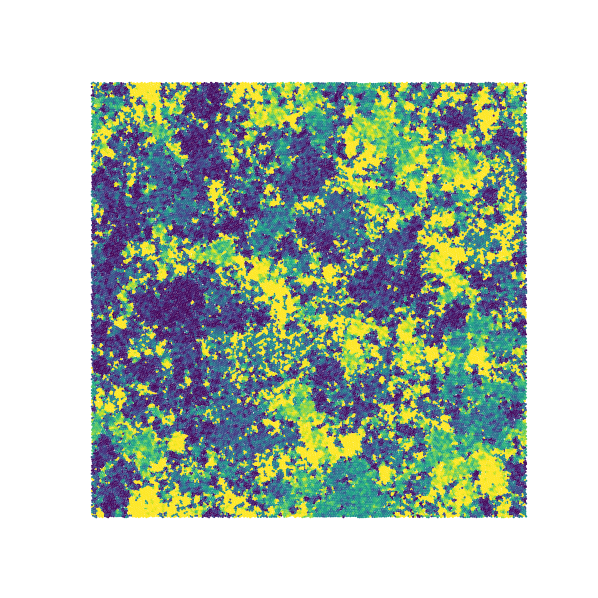
\includegraphics[width=1\columnwidth]{698_-1.png}
	\end{subfigure}\hfil
	\begin{subfigure}[ht]{.33\textwidth}
		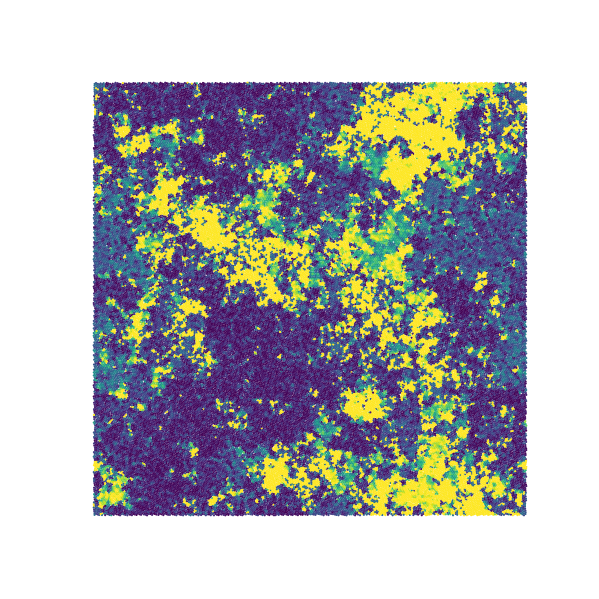
\includegraphics[width=1\columnwidth]{704_-1.png}
	\end{subfigure}\hfil
	\begin{subfigure}[ht]{.33\textwidth}
		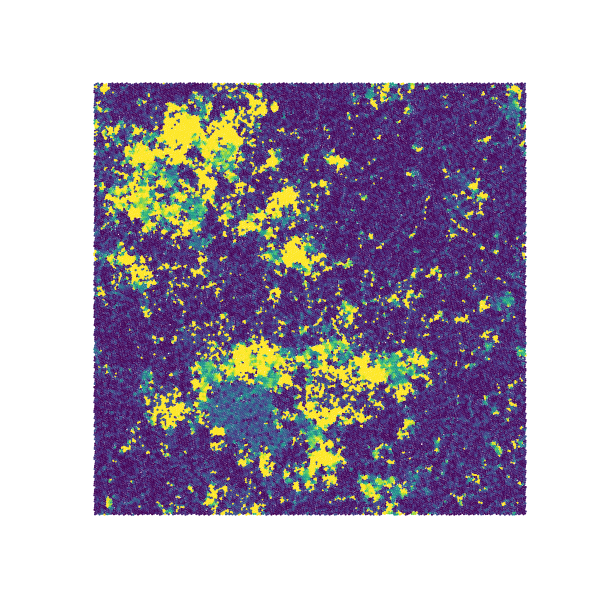
\includegraphics[width=1\columnwidth]{708_-1.png}
	\end{subfigure}
	\medskip
	\begin{subfigure}[ht]{.33\textwidth}
		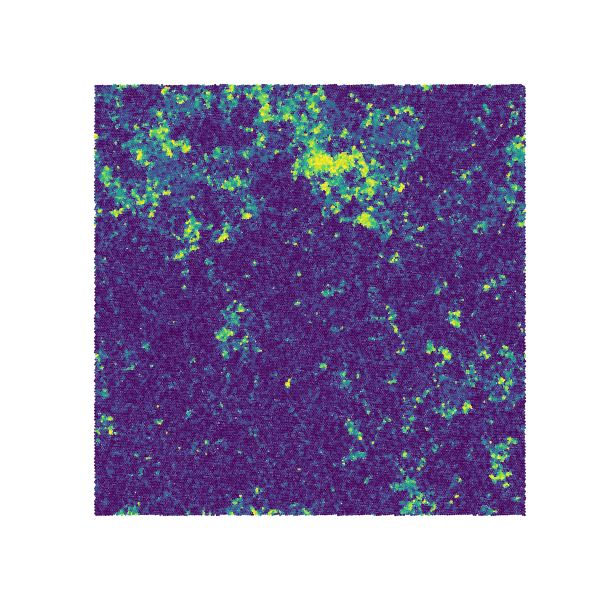
\includegraphics[width=1\columnwidth]{712_-1.png}
	\end{subfigure}\hfil
	\begin{subfigure}[ht]{.33\textwidth}
		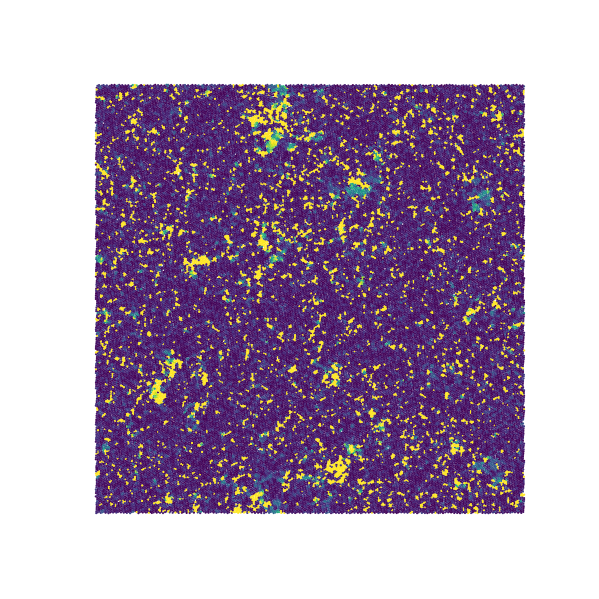
\includegraphics[width=1\columnwidth]{718_-1.png}
	\end{subfigure}\hfil
	\begin{subfigure}[ht]{.33\textwidth}
		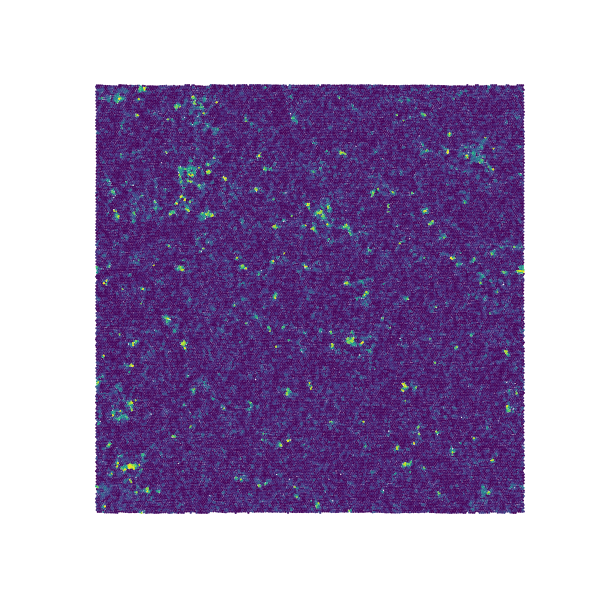
\includegraphics[width=1\columnwidth]{720_-1.png}
	\end{subfigure}
	\caption{
		Local six-fold bond orientational order parameter field of densities: $\phi =$ 0.698, 0.704, 0.708, 0.712, 0.718, 0.720. Each part of the colors represent a different state, and the evolution shows us a transition from the liquid phase to phase coexistence to the hexatic phase. Colors from blue to yellow represent the angle between the local orientations $\Psi_{j,6}$ and the global orientation parameter $\Psi$ from $0$ to $\pi$. 
	}
	\label{fig:psi6}
\end{figure}

Fig.\ref{fig:psi6} shows the local orientations of the system at different densities: $\phi =$ 0.698, 0.704, 0.708, 0.712, 0.718, 0.720. Colors represent the angle between the local orientations $\Psi_{j,6}$ and the global orientation parameter $\Psi$, ranging from $0$(blue) to $\pi$(yellow). We can see that from lower to higher densities, the system goes from a liquid state to phase coexistence states, and finally to a hexatic phase that preserve orientational order over long distances.


\paragraph{Thermodynamic entropy and free energy calculation}

Since quantities like entropy and free energy are not simply averages of functions of the phase space coordinates of the system, it is not possible to measure the free energy or entropy directly in simulation. A common scheme to calculate free energy is based on the thermodynamic equality:
\begin{equation} \label{eq:thermo}
\left(\frac{\partial F}{\partial V}\right)_{N,T} = -p.
\end{equation}
In our hard-disk system, to compute the free energy at a given desity, we should find a reversible path that links the target state to a state of known free energy, and the change of F along that path can then be evaluated by thermodynamic integration of Eq.\ref{eq:thermo}. In general, for fluid state, we can choose the reference state to be ideal gas, and the excess free energy, which is the difference between the two states, is given by \cite{PhysRevE.93.012906}:
\begin{equation} \label{eq:F}
f_{ex}(\rho) = \frac{F(\rho)}{N} - \frac{F^{id}(\rho)}{N} = \int_{0}^{\rho} d\rho'\left[\frac{p(\rho') - \rho'}{\rho'^2}\right].
\end{equation}
While for solid state, if the integration path crosses a strong first-order phase transition, such as the melting transition in three dimension, hysteresis may occur and the path is irreversible, we can no longer use the ideal gas as reference state and integrate from liquid state. Instead, we would have to compute the free energy on the solid side by the Frenkel-Ladd method, using Einstein crystal whose free energy is known as our reference state \cite{frenkel2001understanding}.

However, in our case of two-dimensional melting, it is safe to integrate from the liquid part directly because unlike in three dimension, the transition is very weakly first order. Here since we only have a segment of equation of state near the transition, it is reasonable to just simply integrate the region we have. The entropy we get from this calculation will only differ by a trivial constant compared with the absolute entropy. The blue lines in Fig.\ref{fig:phi_cid_grid} and Fig.\ref{fig:p_cid_grid} are the integrated thermodynamic entropy S plotted as a function of volume fraction $\phi$ and pressure $p$ respectively from the polynomial fit of the EOS as we mentioned before.

Alternatively, to do this right quantitatively we would have to integrate the analytical equation of state from the ideal gas up to the lowest density point we have measured, and then use the data we have to cover the transition region, which will give us the absolute value of the entropy. 


\begin{figure}[ht]
	\begin{subfigure}[ht]{.5\textwidth}
		\centering 
		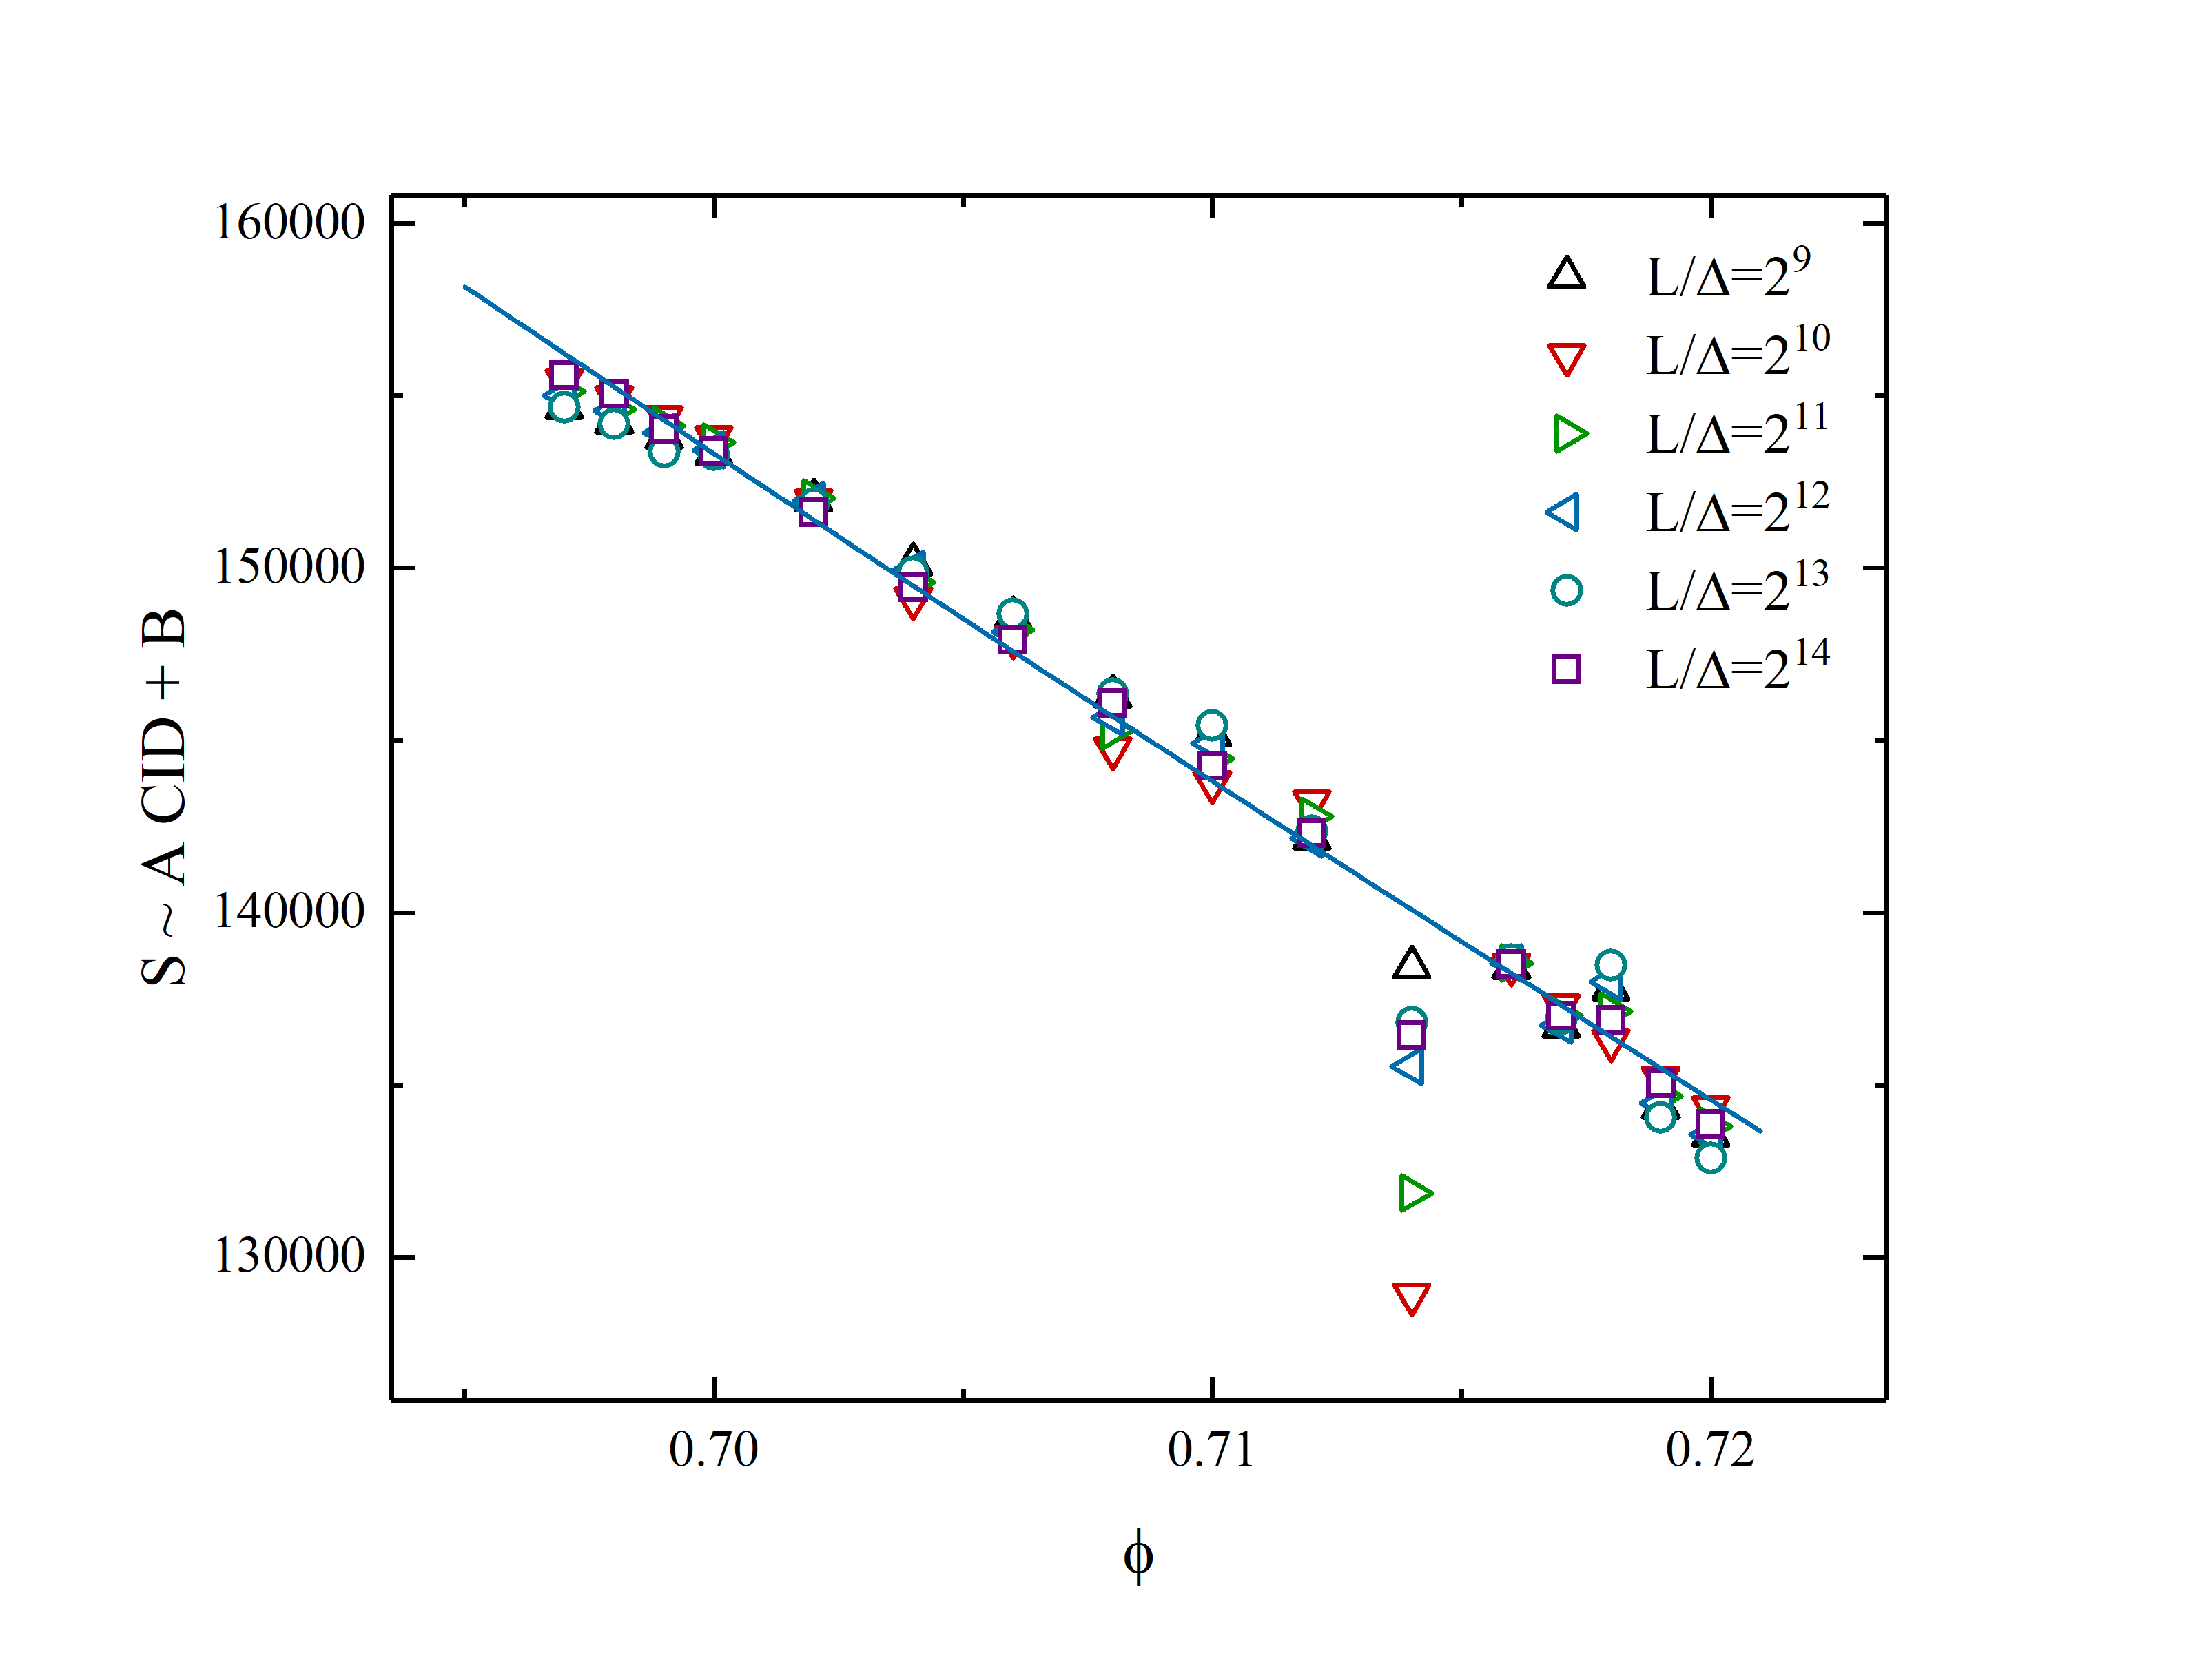
\includegraphics[width=1\columnwidth]{phi_cid_grid.png}
		\caption{}
		\label{fig:phi_cid_grid}
	\end{subfigure}
	\begin{subfigure}[ht]{.5\textwidth}
		\centering
		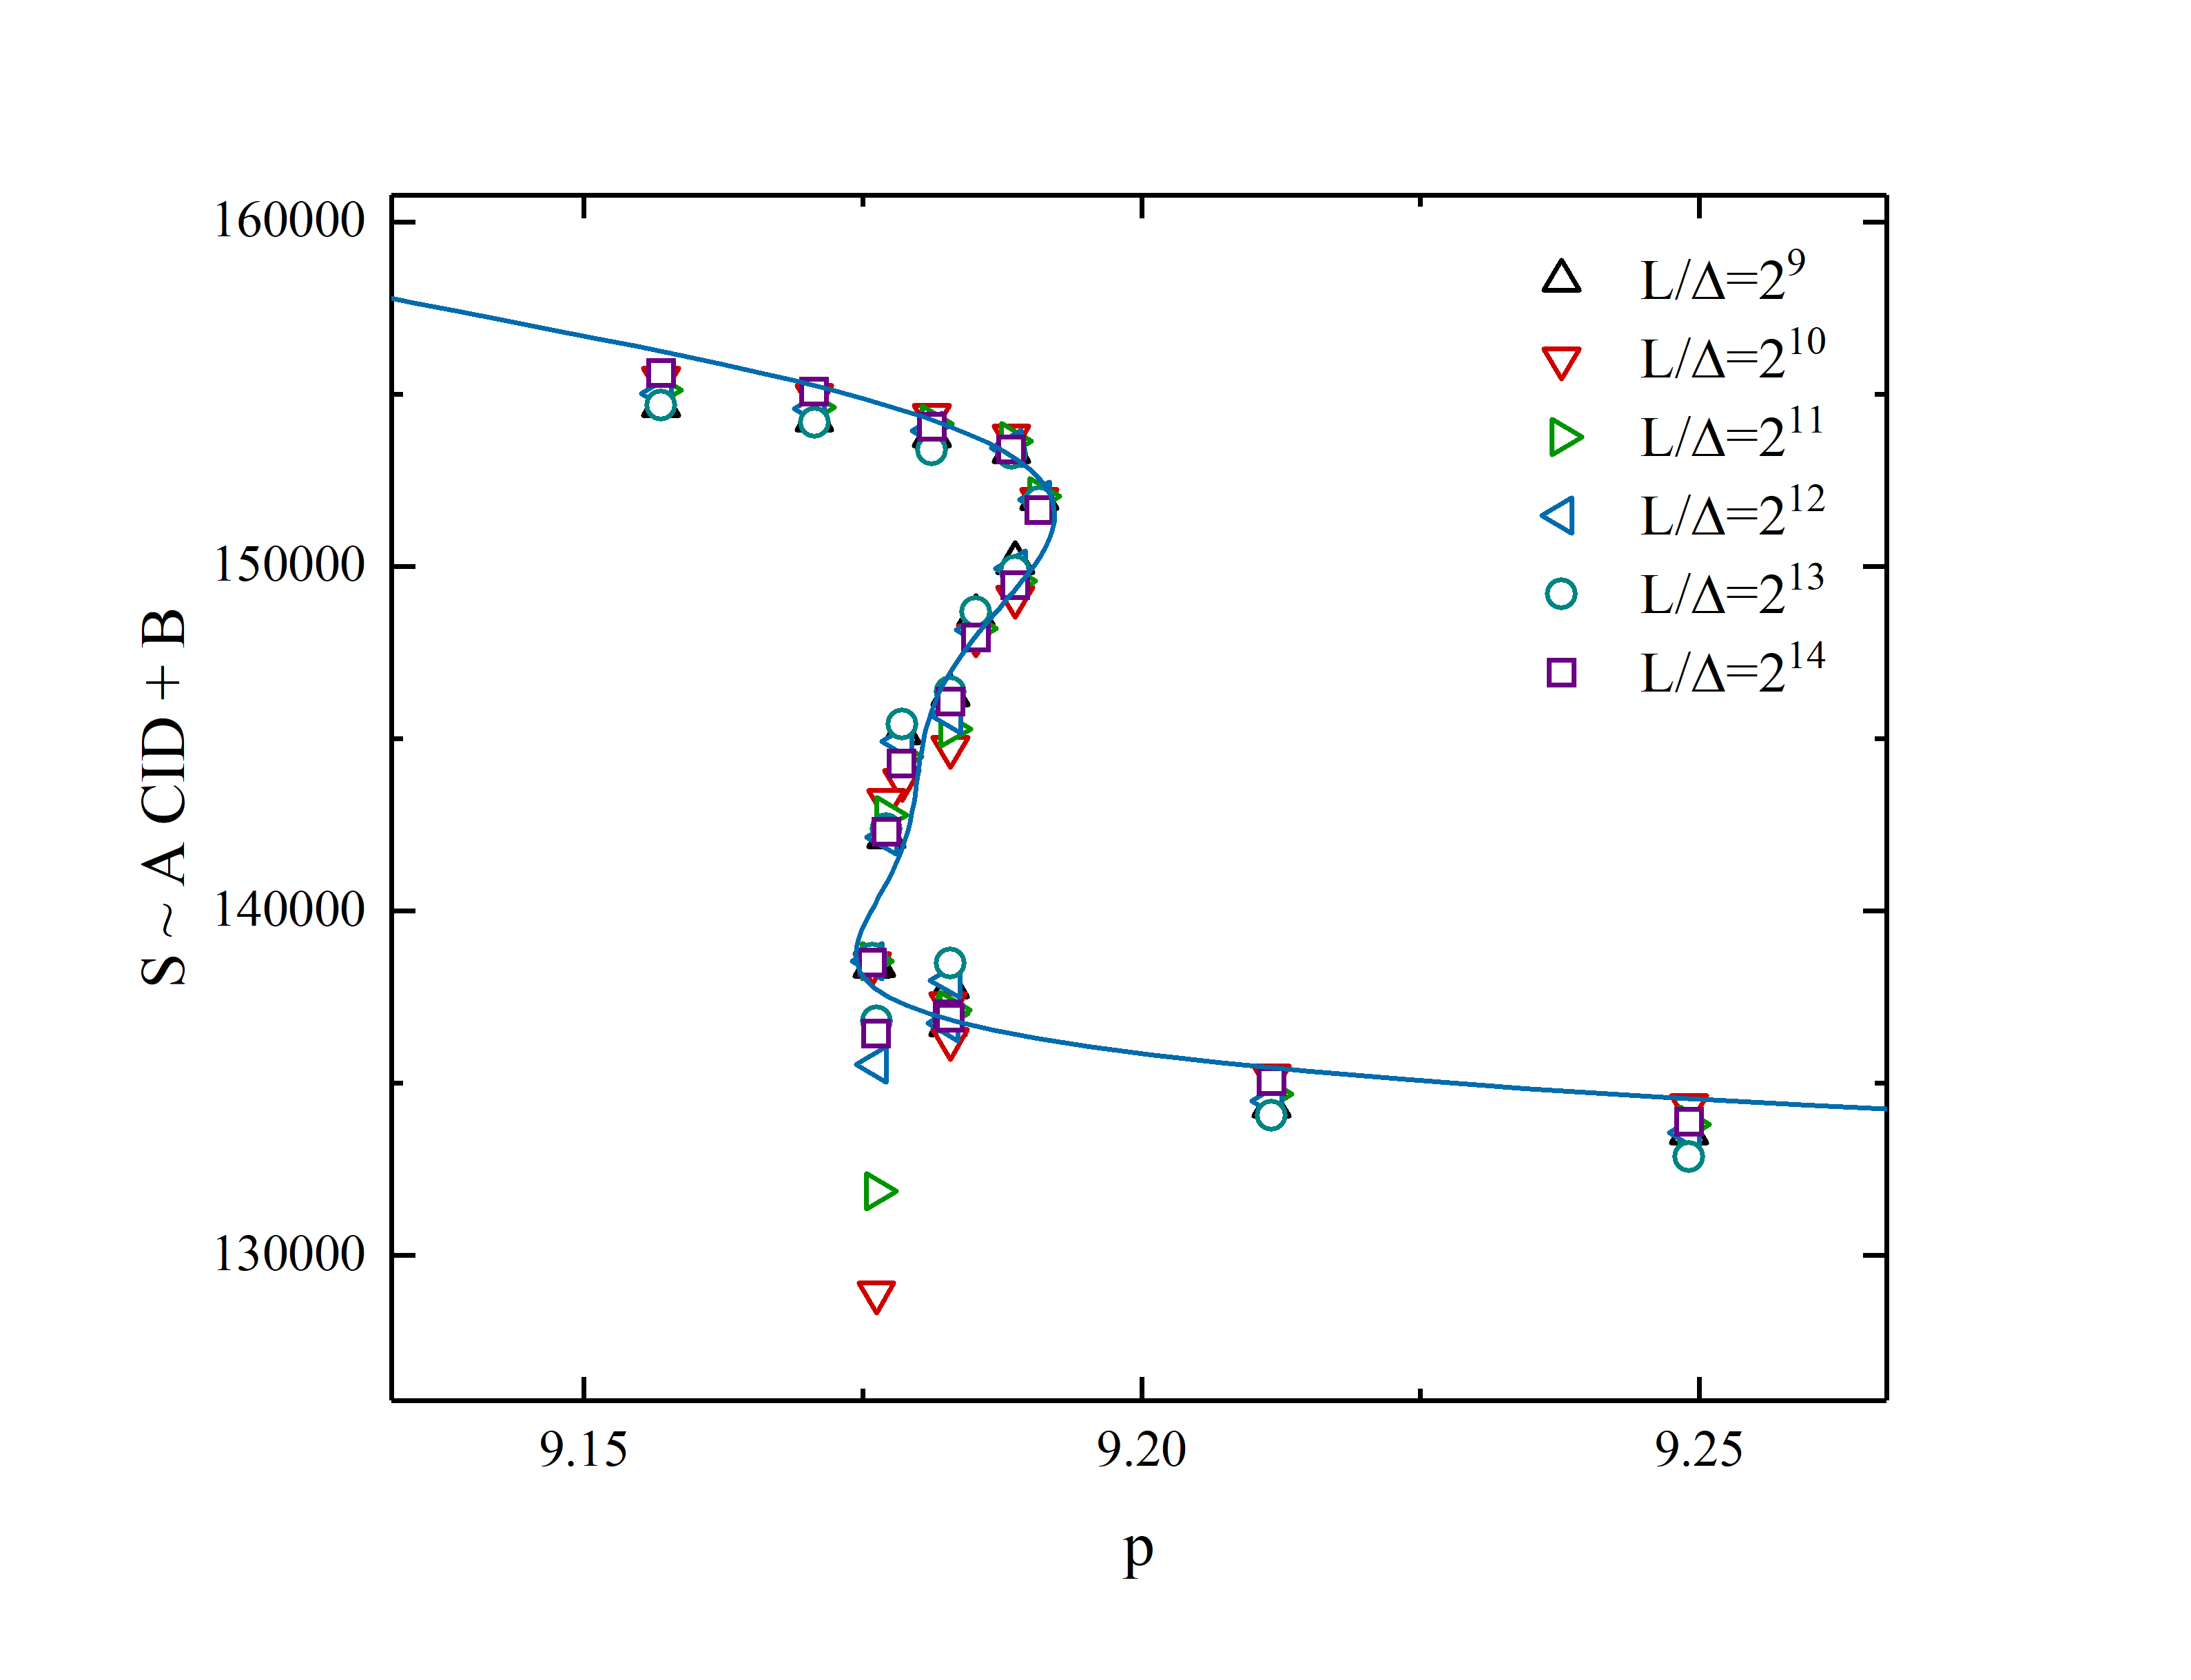
\includegraphics[width=1\columnwidth]{p_cid_grid.png}
		\caption{}
		\label{fig:p_cid_grid}
	\end{subfigure}
	\caption{
		 Entropy of hard-disk system near the melting transition with control variable: (a) volume fraction $\phi$, (b) pressure $p$. The blue lines are thermodynamic entropy calculated by  integrating the fitted equation of state. Data points are the linear collapse of CID calculated with different coarse-graining bin size $L/\Delta$ ranging from $2^9$ up to $2^{14}$ for the $N=256^2$ system.
	}
	\label{fig:cid_grid}
\end{figure}


\paragraph{Information entropy and data compression}

One important concept in information theory is the Shannon entropy, which gives a quantitative measure of the information content
and order of a system. It is commonly explained in the context of a sequence $x$ of length n. In this case, the Shannon entropy $H(X)$ is defined as
\begin{equation}
H(X)=-\sum_{\{x\}} p(x) \log_2 p(x),
\end{equation}
where the $\{x\}$ runs over all possible bit sequences of length n and $p(x)$ is the probability of sequence $x$ occurring.

For systems in equilibrium, it can be easily seen from the concept of Gibbs entropy $S=-k_B \sum p_i \ln p_i$ in statistical thermodynamics that the Shannon entropy and the thermodynamic entropy are equivalent, apart from a factor of $\ln 2$. In this term, $x$ can be viewed as microstates and the probabilities of their occurrence $p(x)$ are simply the Boltzmann weights: $p(x)=\exp(-\beta E(x))/Z$, where $E(x)$ is the energy of state $x$, and $Z$ is the partition function. 

According to Shannon’s source coding theorem, which states that in
the large system limit, the size of the shortest encoding that can be achieved without loss of information is the entropy H. Thus an optimal universal data compression algorithm may be used to approximate Shannon entropy. In this work, we employ the Lempel Ziv string-matching algorithm (LZ77) for data compression, which searches for repeating data patterns (the longest previous factor) in the previous sequence and stores it with tuples representing the position and length of the matching subsequence. The total binary code length for LZ77 algorithm is approximated as \cite{2017arXiv170804993M}
\begin{equation} \label{eq:length}
\mathscr{L} \approx C \log C + 2 C \log \frac{L}{C}, 
\end{equation}
where C is the number of the longest previous factor, L is the length of the original sequence. The Computable Information Density (CID), which is an estimator for the true Shannon entropy, is defined as:
\begin{equation} \label{eq:CID}
{\rm CID} \equiv \frac{\mathscr{L}(x)}{L}.
\end{equation}
Since CID converges to $H$ as $L \to \infty$, we will use CID as an approximation of information entropy later.

In order to examine the behavior of CID during the phase transition and how it is related with the true thermodynamic entropy, we calculated the averaged CID for each density by converting the configurations to sequences of binary data in the order along Hilbert curve, which can actually work for arbitrary dimension using the scheme involving bitwise operations embedded in the package \textit{sweetsourcod}. Specifically, we divided the simulation box into discrete pixels grids of $2^n \times 2^n$, and the grids containing the center of a particle is set to be 1, and otherwise 0. In this way, a sequence of data is constructed out of a given particles configuration. Denoting the length of the box to be $L$ and the griding bin size is $\Delta$, we compute the CID as in Eq.\ref{eq:CID} for different values of $L/\Delta$ ranging from $2^9$ up to $2^{14}$ for our $N=256^2$ system size. These kind of discretization is in fact a coarse-graining issue that introduce systematic errors, and from the concept of discrete entropy and differential entropy \cite{Cover:2006:EIT:1146355}, we expect to see a convergence of the CID with different $\Delta$ to some kind of differential entropy that may relate directly to the thermodynamic entropy S. To find out the relation, we here impose the optimal linear mapping: $S = A(\Delta)~ {\rm CID} + B(\Delta)$ that collapses CID into our measures thermodynamic entropy as shown in Fig.\ref{fig:cid_grid}.

\begin{figure}[ht]
	\begin{subfigure}[ht]{.5\textwidth}
		\centering 
		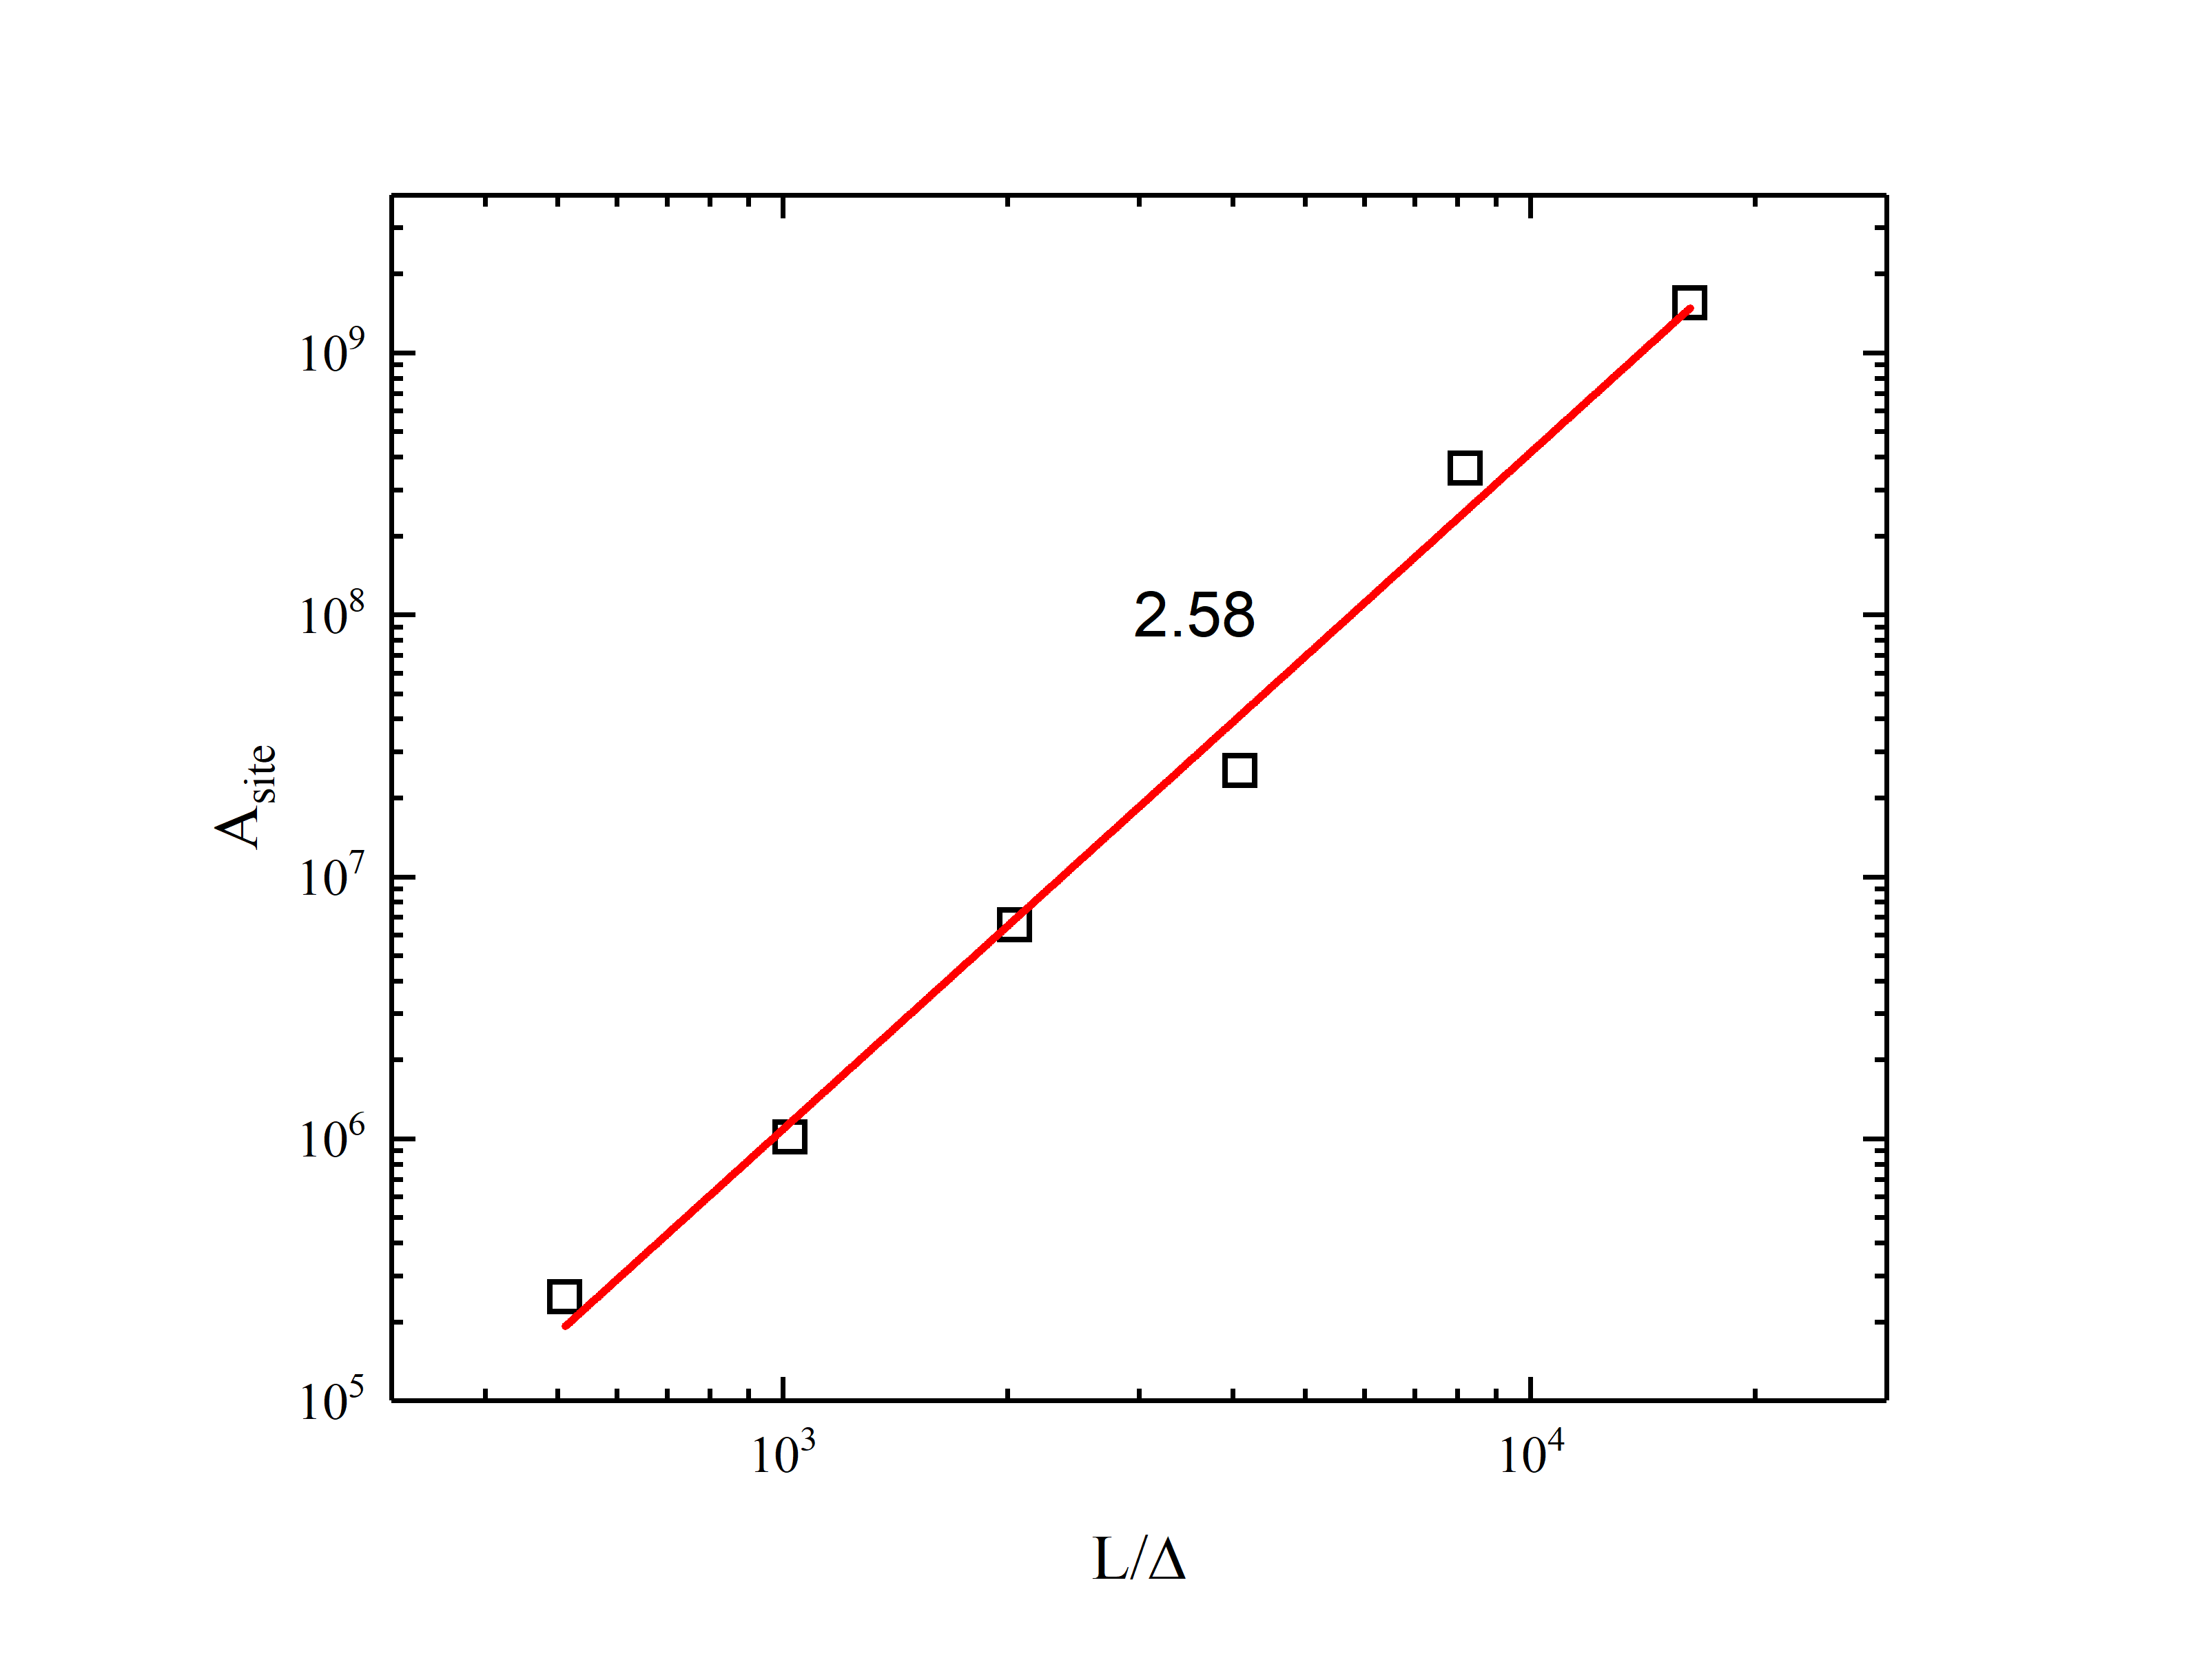
\includegraphics[width=1\columnwidth]{Asite.png}
		\caption{}
		\label{fig:Asite}
	\end{subfigure}
	\begin{subfigure}[ht]{.5\textwidth}
		\centering
		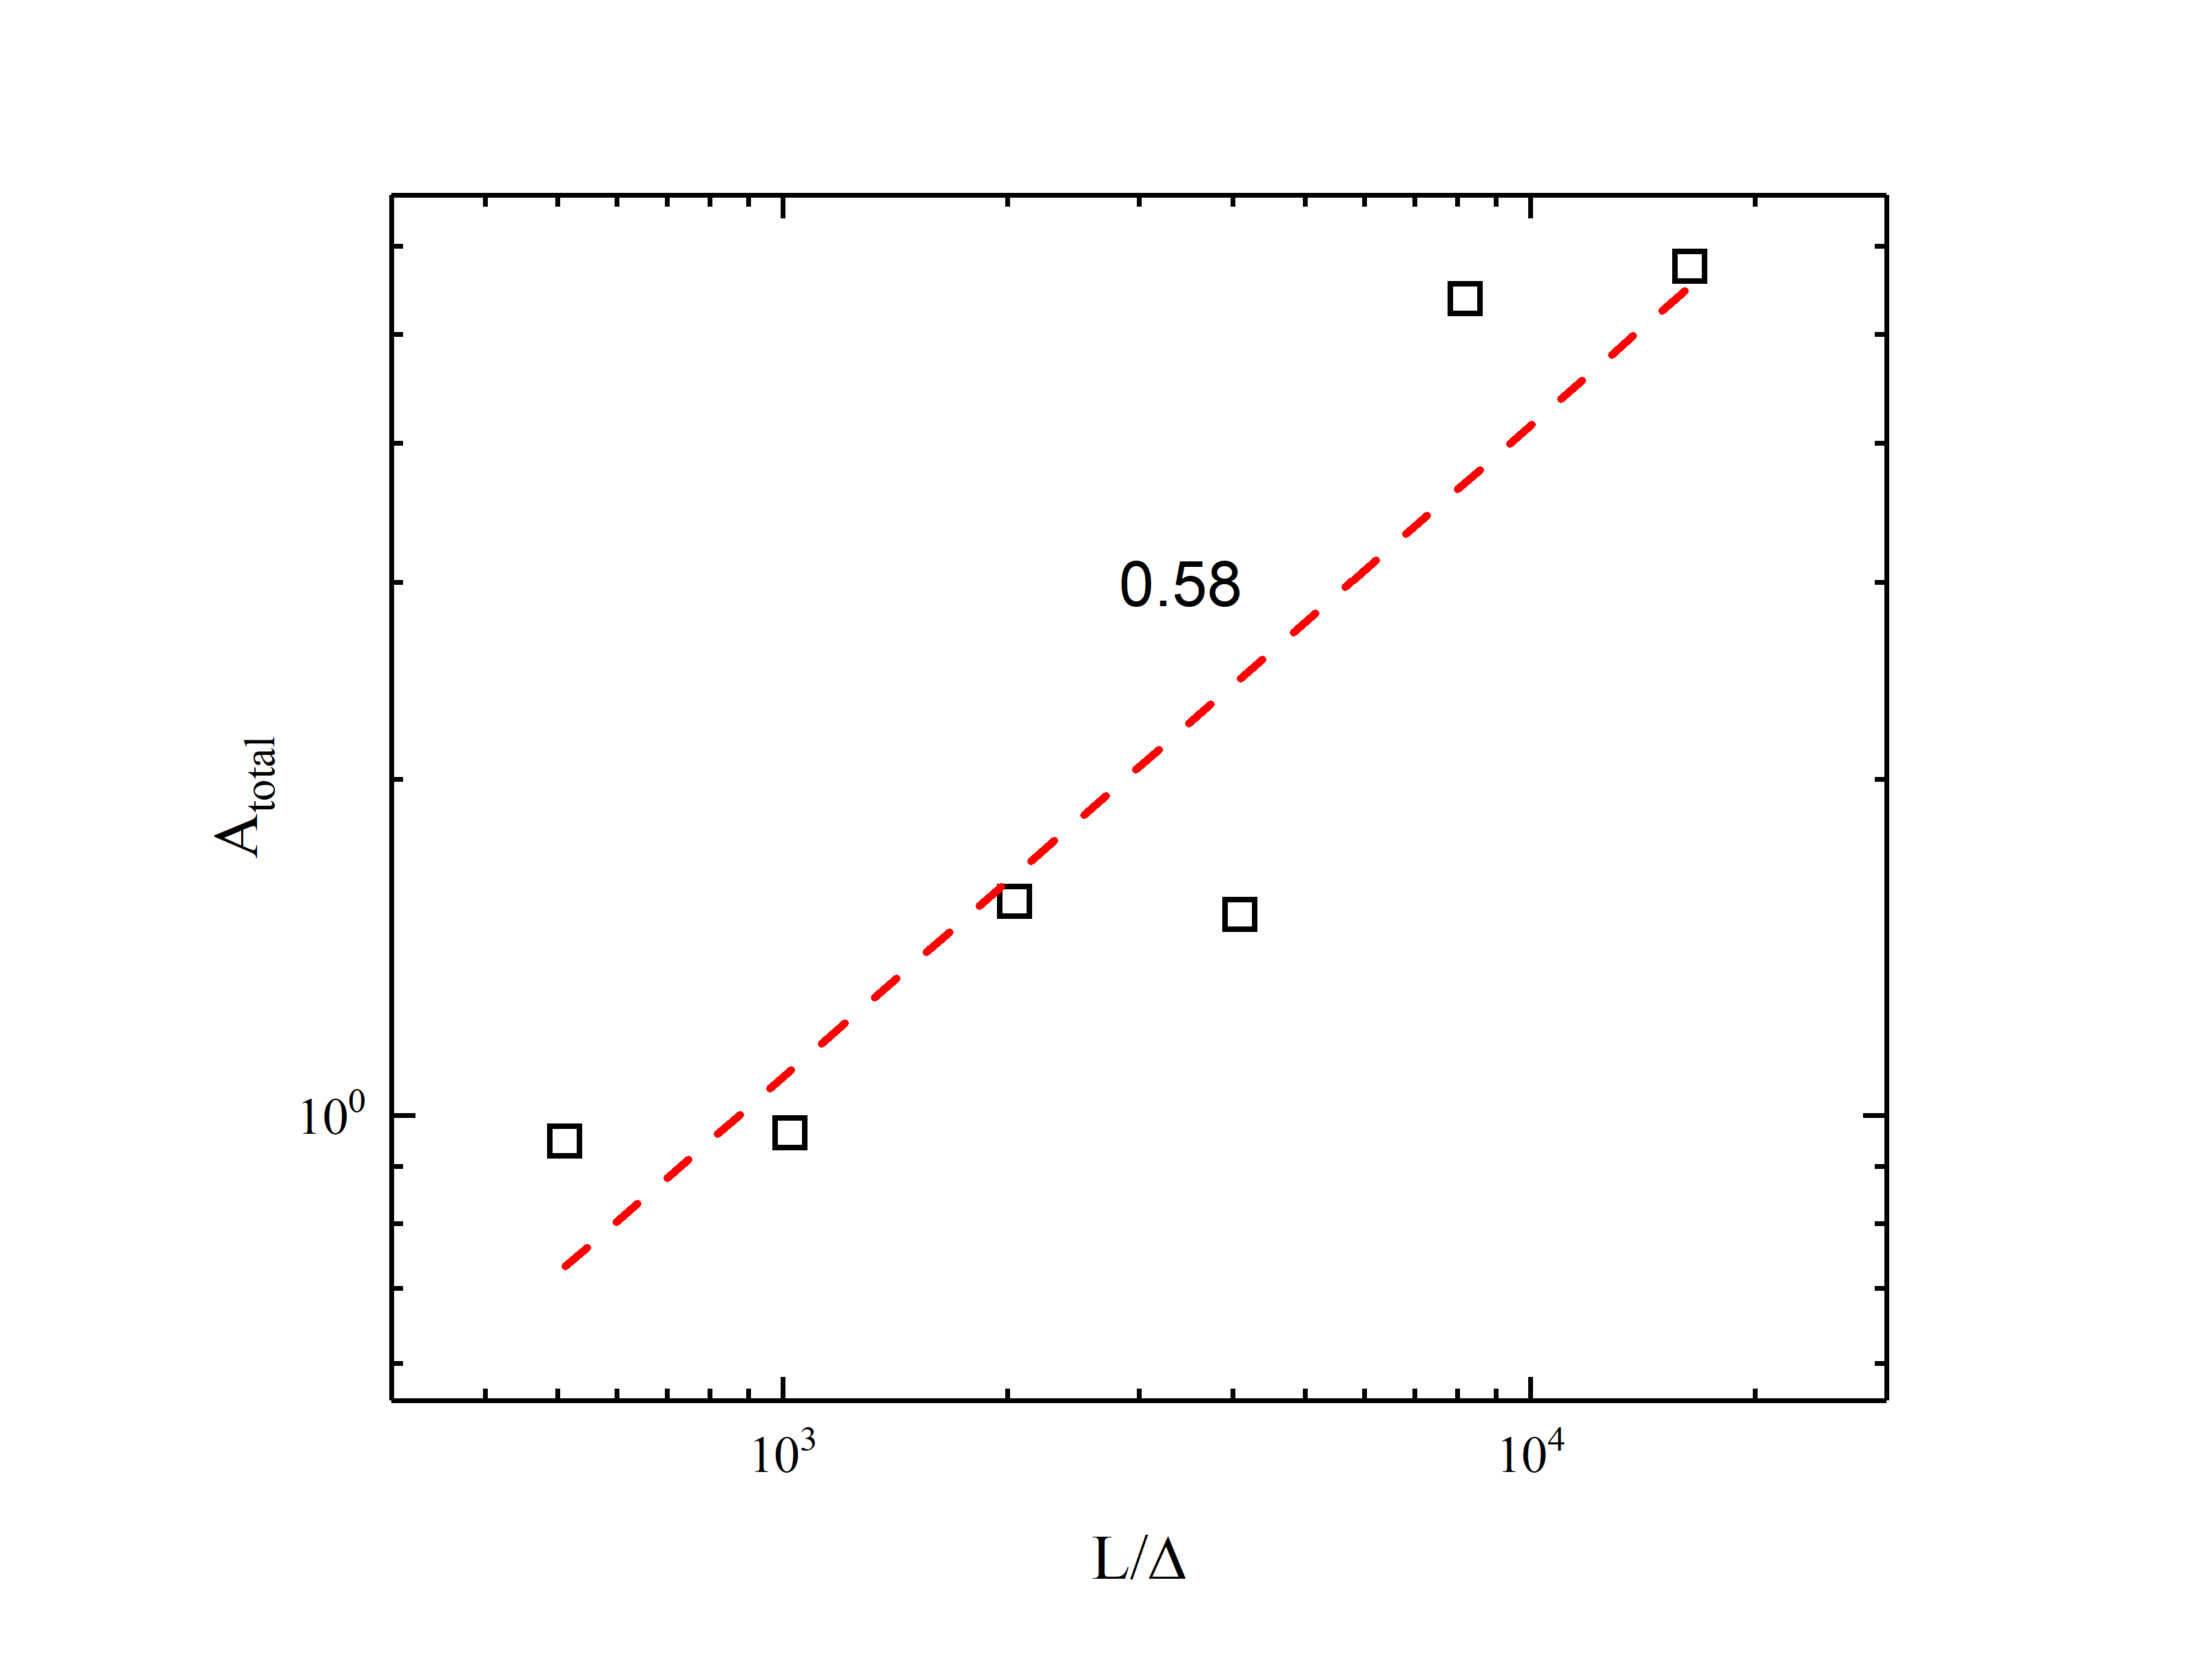
\includegraphics[width=1\columnwidth]{Atot.png}
		\caption{}
		\label{fig:Atot}
	\end{subfigure}
	\caption{
		 The optimal linear mapping coefficients from CID to thermodynamic entropy with respect to the number of bins in each dimension $L/\Delta$, where the CID is taken as CID per site in (a) and the total CID in (b). We have the scaling relation of $A_{site} \sim (L/\Delta)^{2.58}$ and $A_{total} \sim (L/\Delta)^{0.58}$.
	}
\end{figure}

The mapping coefficients $A(\Delta)$ is the one we are concerning about, while $B(\Delta)$ is just a difference of constant of the entropy. The relation is demonstrated in Fig.\ref{fig:Asite} and Fig.\ref{fig:Atot}, where the CID is taken as the CID per site (same as in Eq.\ref{eq:CID}) and the total CID ($\mathscr{L}$ in Eq.\ref{eq:length}) separately. The scaling relation of $A_{site} \sim (L/\Delta)^{2.58}$ or $A_{total} \sim (L/\Delta)^{0.58}$ may depend on dimensionality, and the reasons for this result remains to
be explored.

\paragraph{Discussion}

At present stage, we have determined and visualized hard-disk melting transition. To examine how well data compression scheme can represent the thermodynamic entropy of a system, we also tried to relate these two quantities during the transition. However, it may not seem to be so convincing to tell that CID to entropy is a linear mapping because the region we currently measure is quite narrow. To make it more precise, we should next take more points from relatively lower density in liquid to higher density in solid across the transition area to see the exact relation. Also we should better follow the method mentioned before to obtain the absolute value of thermodynamic entropy rather the one that differs by a constant.

\begin{figure}[ht]
	\begin{subfigure}[ht]{.5\textwidth}
		\centering 
		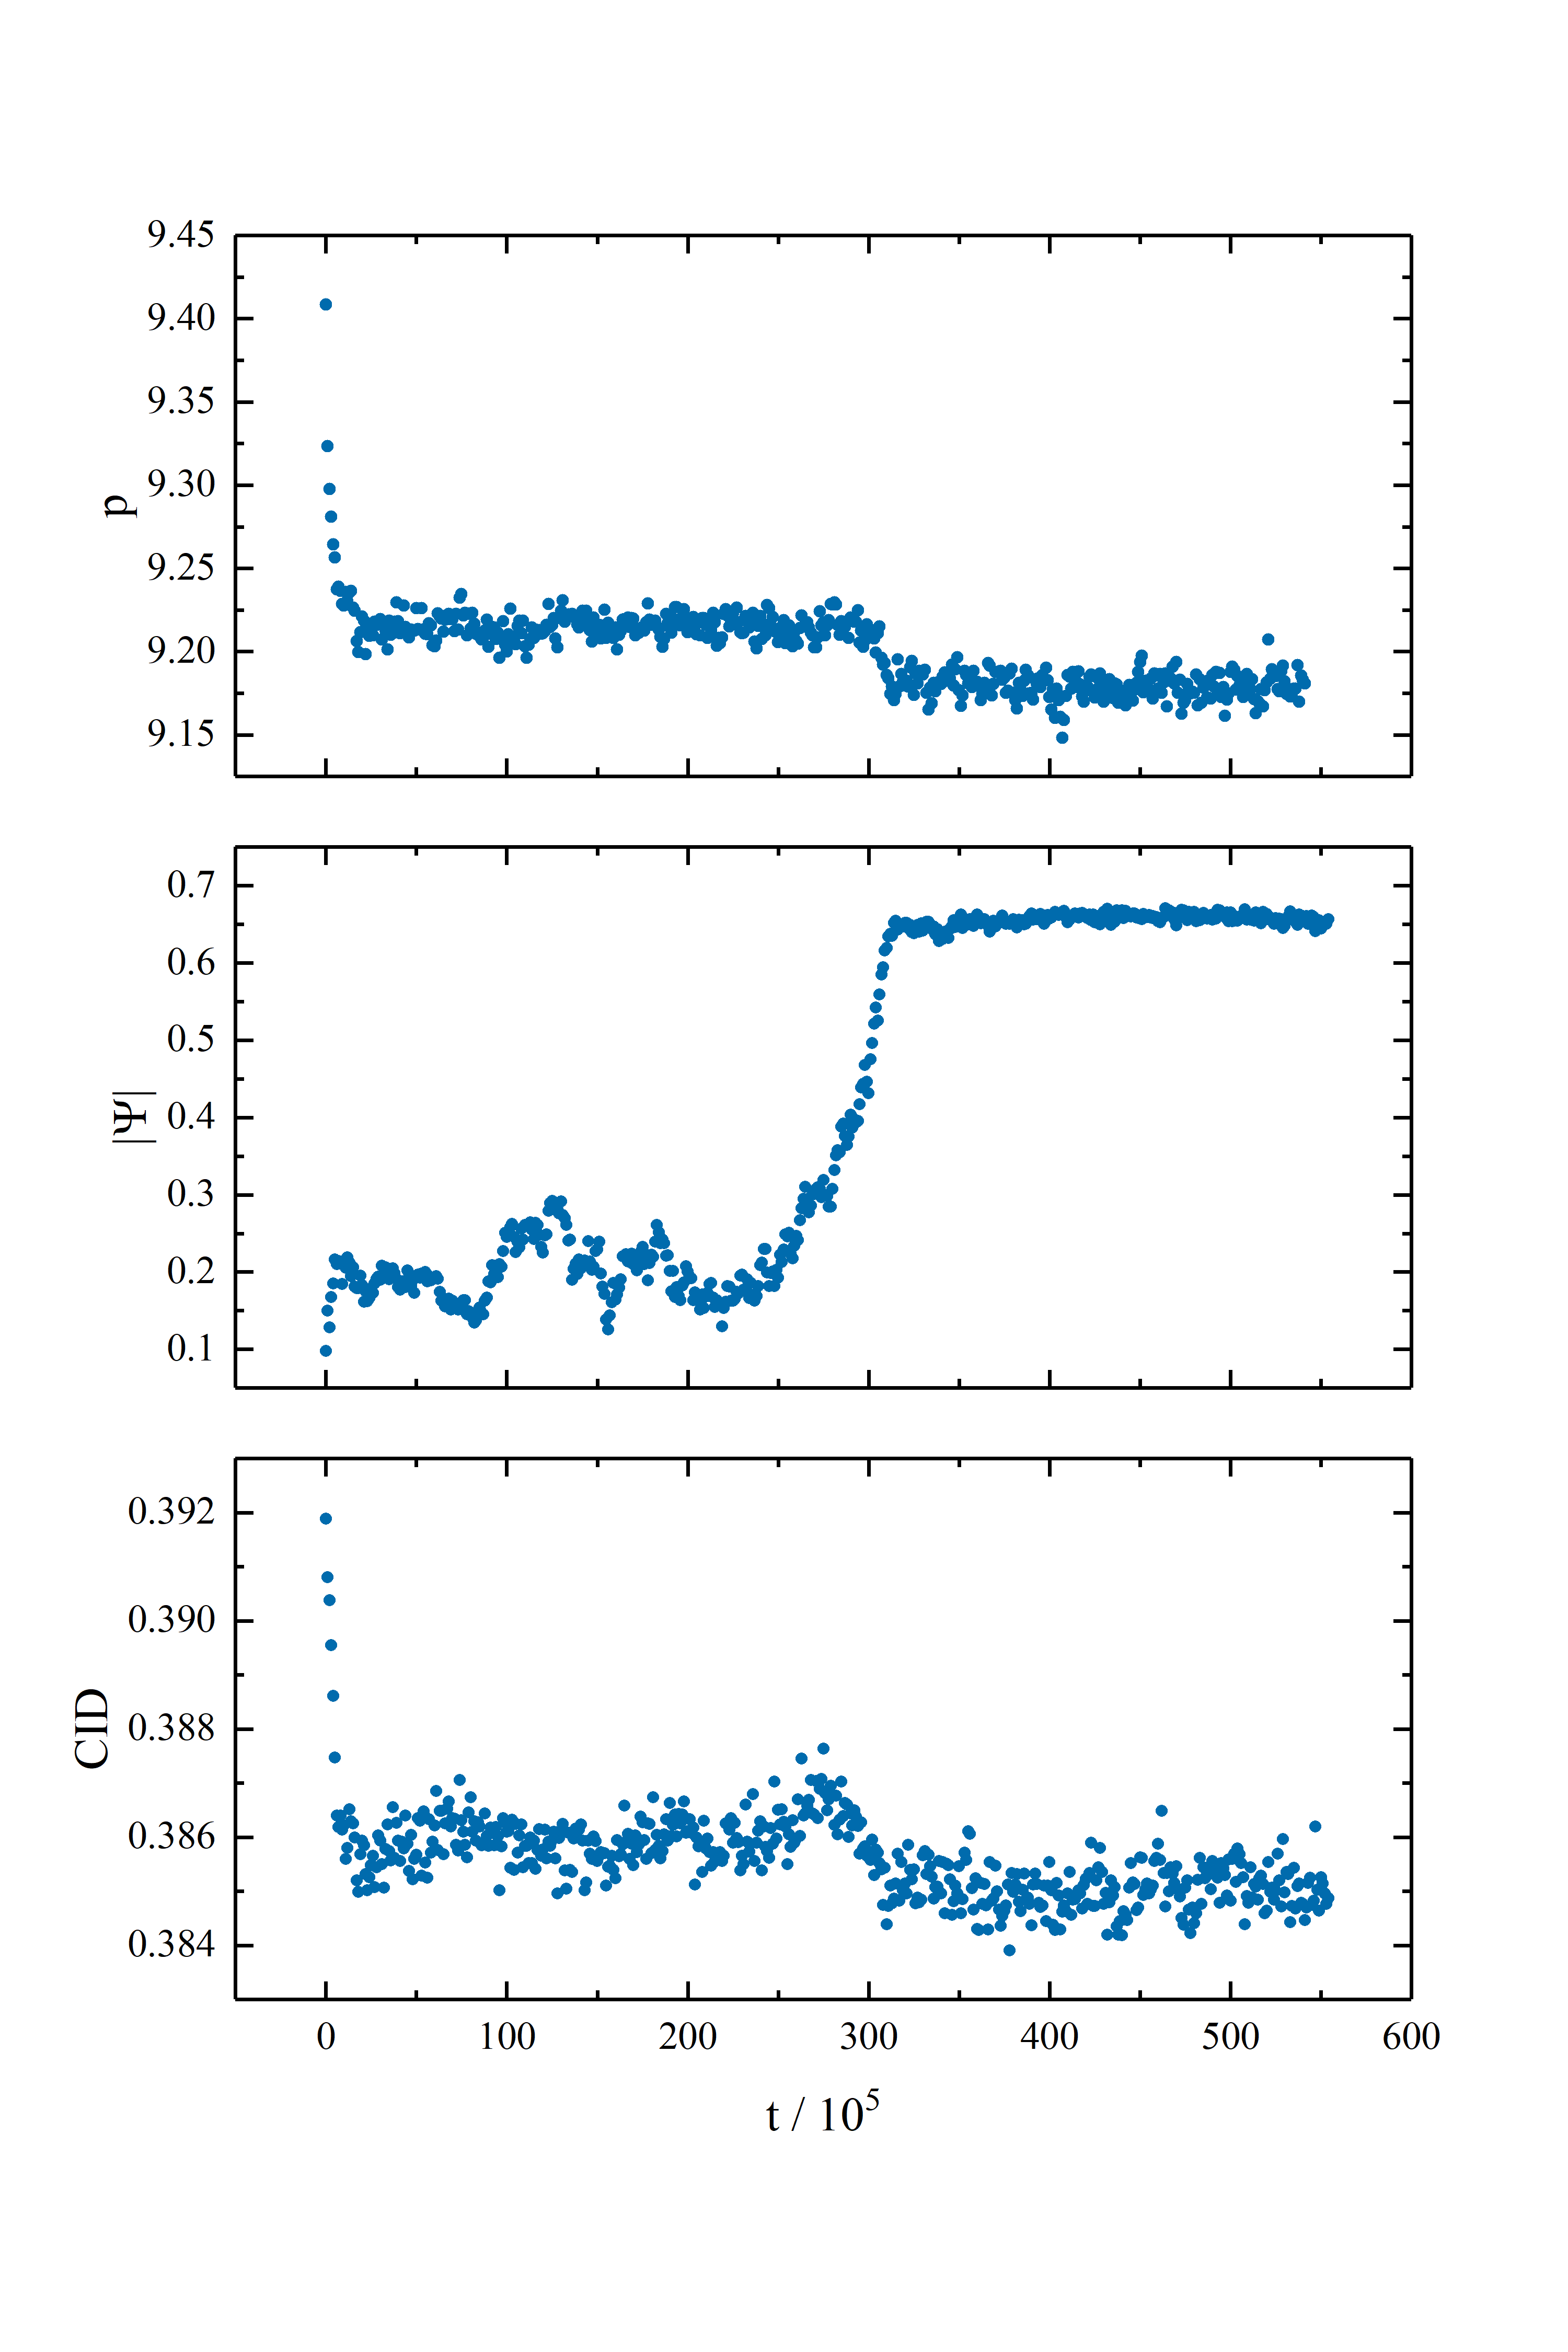
\includegraphics[width=1\columnwidth]{t_evo_714.png}
	\end{subfigure}
	\begin{subfigure}[ht]{.5\textwidth}
		\centering
		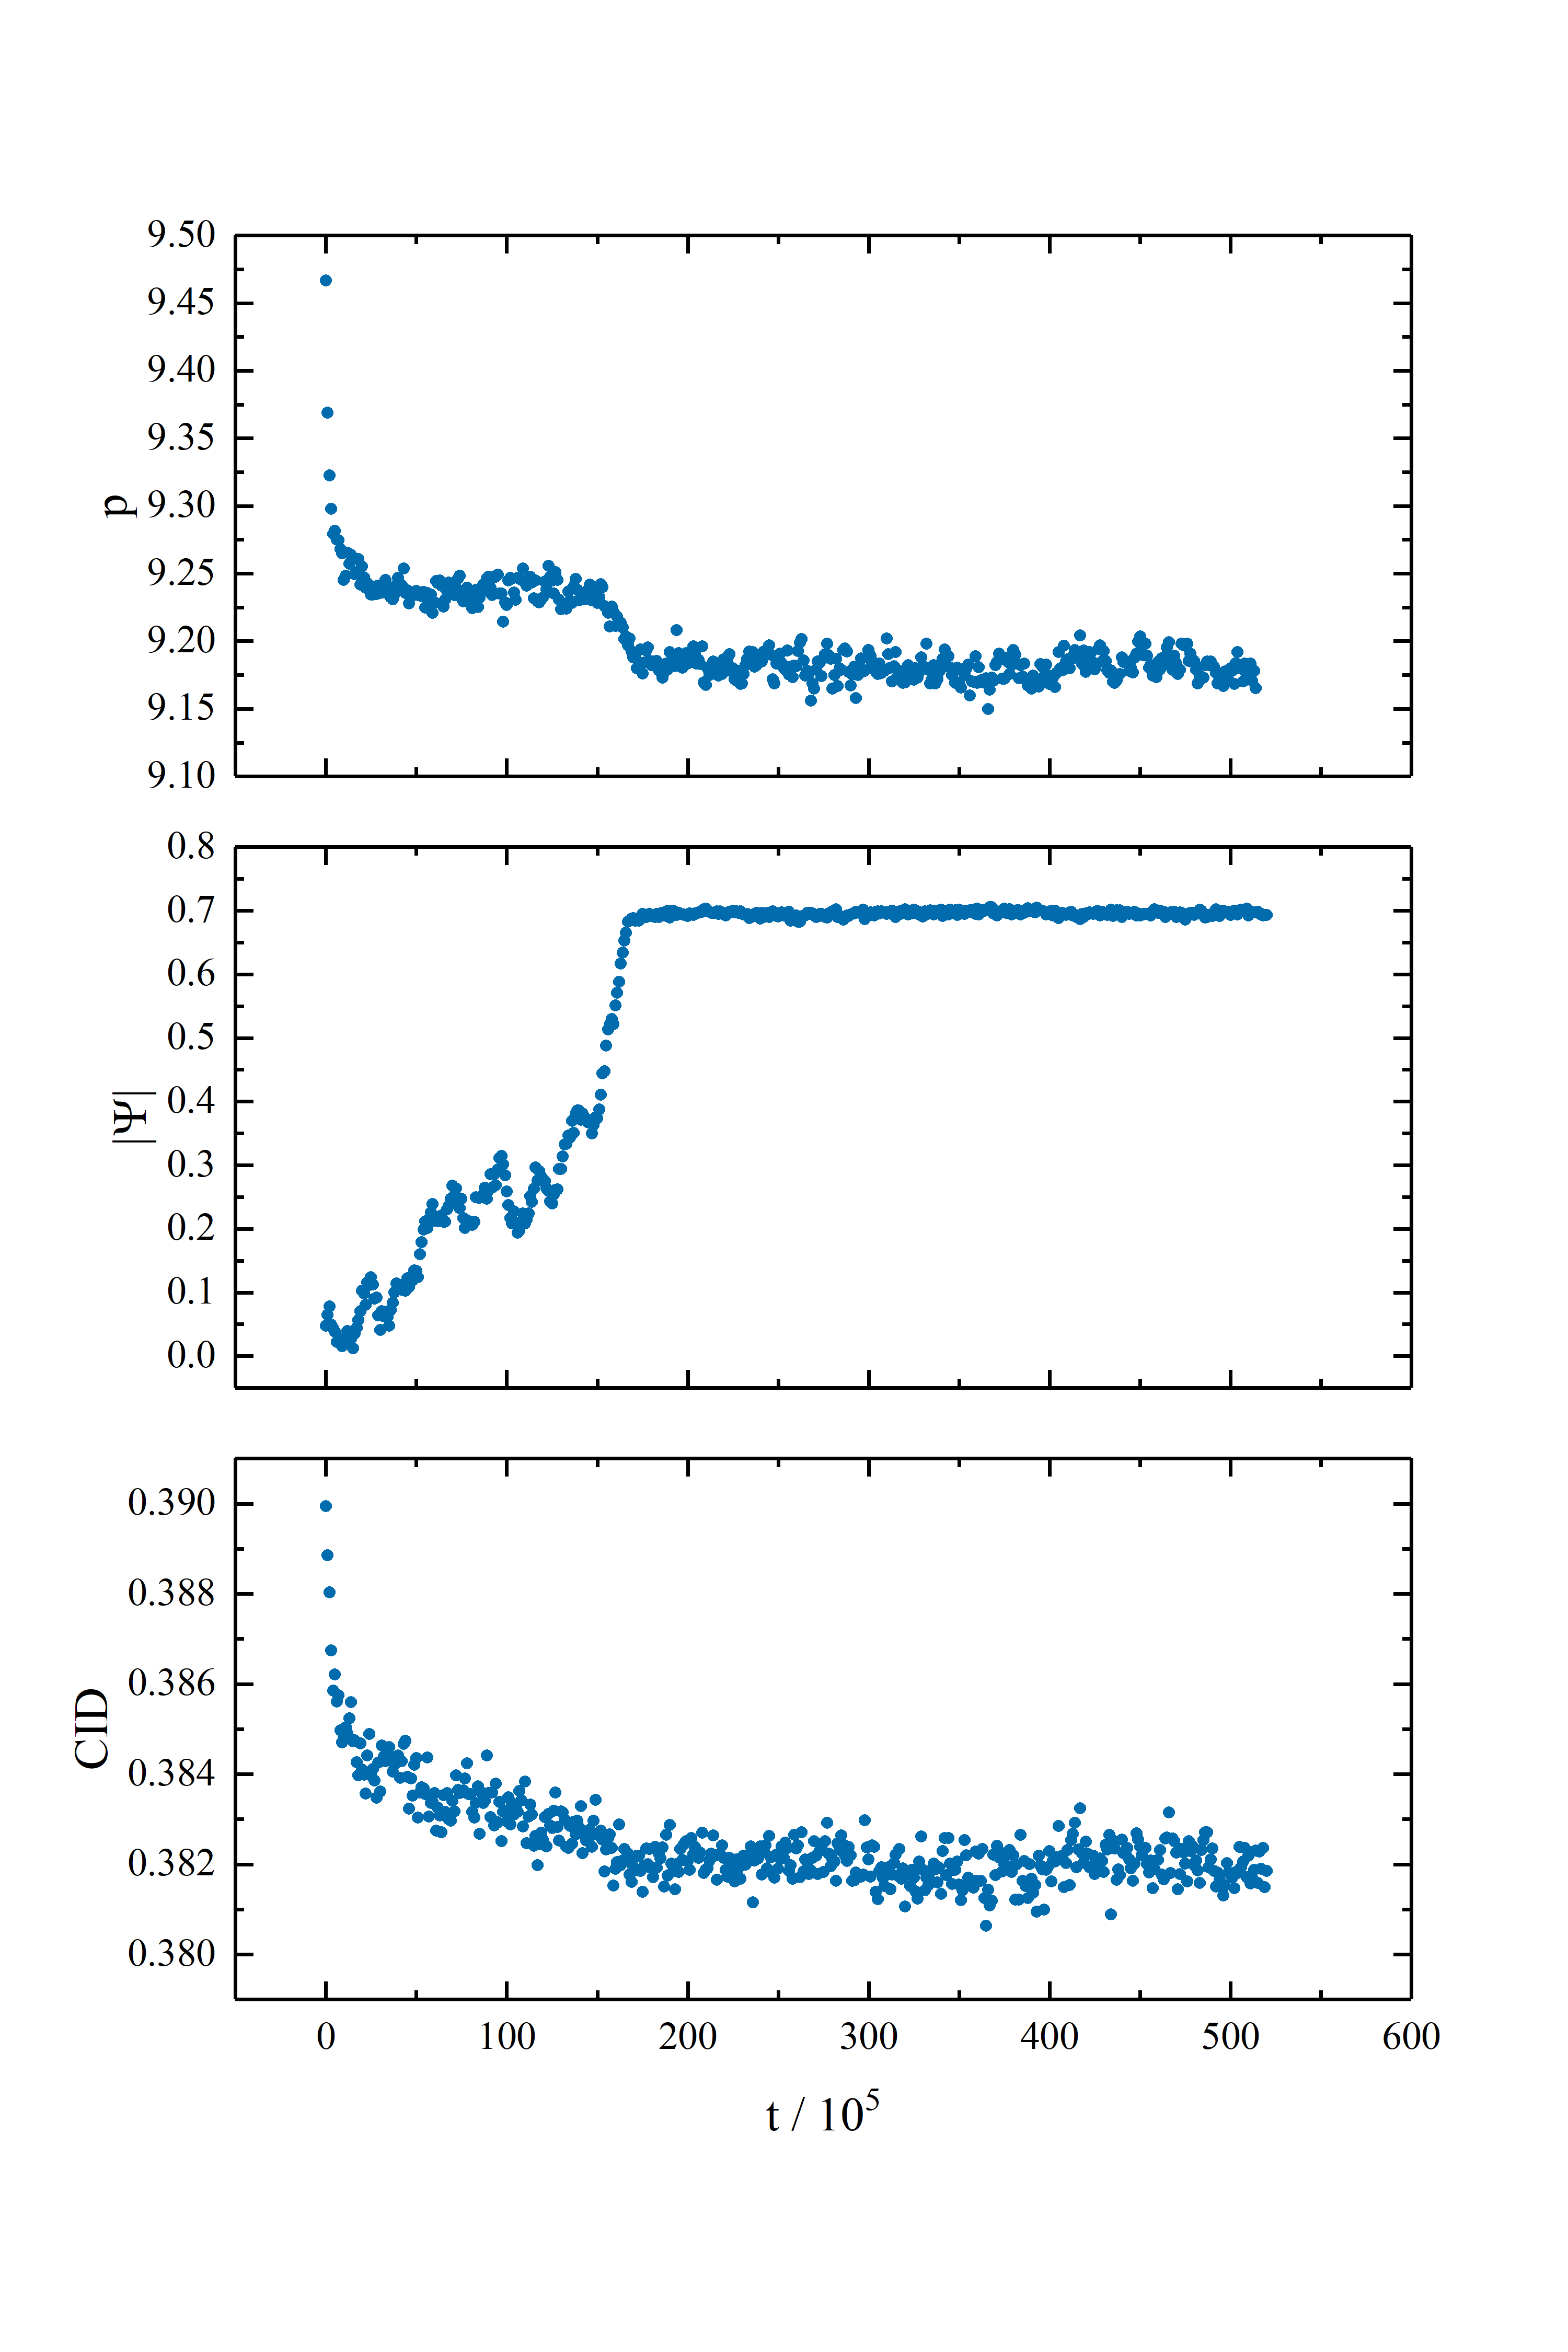
\includegraphics[width=1\columnwidth]{t_evo_716.png}
	\end{subfigure}
	\caption{
		The time evolution of pressure $p$, global bond orientational order $|\psi|$ and the CID in the process of evolving from a initial non-equilibrium state to the final equilibrium state. Left and right panels are taken from two different densities $\phi=$0.714 and 0.716.
	}
	\label{fig:t_evo}
\end{figure}

The concept of thermodynamic entropy is well define in a system in equilibrium, while the CID is valid both in and out of equilibrium. The entropy and CID of melting transition we were discussing are all taken when the system is in thermodynamic equilibrium, and now we briefly take a look at the time evolution process towards equilibrium. In Fig.\ref{fig:t_evo}, we check for two densities $\phi=$0.714 and 0.716, where there is a significant transition from a non-equilibrium state to the final equilibrium as can be observed directly from both the pressure and the global orientational order parameter. The CID, however, seems to have a precursor in the $\phi=0.714$ case, while in the other, it only shows a discontinuity of the slope. These kind of different behavior of CID in a similar transition still requires further exploration.


\section*{Acknowledgments}

I would like to thank Stefano Martiniani and Paul Chaikin for instruction and advising. I would also like to thank High Performance Computing (HPC) at NYU for computing time and resource. 

\bibliography{hd}

\end{document}